\documentclass[11pt,a4paper]{article}

% ================= PACKAGES =================
\usepackage[a4paper,margin=2.5cm]{geometry}
\usepackage[utf8]{inputenc}
\usepackage[T1]{fontenc}
\usepackage{titlesec}
\usepackage{graphicx}
\usepackage{xcolor}
\usepackage{listings}
\usepackage{booktabs}
\usepackage{longtable}
\usepackage{array}
\usepackage{enumitem}
\usepackage{fancyhdr}
\usepackage{hyperref}
\usepackage{amsmath}
\usepackage{tikz}
\usetikzlibrary{positioning, arrows.meta, shapes.geometric}
\usepackage{pgfplots}
\pgfplotsset{compat=1.18}
\usepackage{caption}
\usepackage{float}
\usepackage{colortbl} % For professional colored tables

% ================= COLORS =================
\definecolor{codebg}{RGB}{248,249,250}
\definecolor{codekeyword}{RGB}{0,51,204}
\definecolor{codecomment}{RGB}{0,128,0}
\definecolor{codestring}{RGB}{163,21,21}
\definecolor{telkomred}{RGB}{198,40,40}
\definecolor{charcoal}{RGB}{50,50,50}
\definecolor{tableheader}{RGB}{240,242,245}

% ================= HYPERREF STYLE =================
\hypersetup{
    colorlinks=true,
    linkcolor=telkomred,
    filecolor=telkomred,      
    urlcolor=telkomred,
    citecolor=charcoal,
}

% ================= LISTING STYLE =================
\lstdefinestyle{pythonstyle}{
    backgroundcolor=\color{codebg},
    basicstyle=\ttfamily\footnotesize\color{charcoal},
    keywordstyle=\color{codekeyword}\bfseries,
    commentstyle=\color{codecomment}\itshape,
    stringstyle=\color{codestring},
    numbers=left,
    numberstyle=\tiny\color{gray},
    stepnumber=1,
    numbersep=8pt,
    breaklines=true,
    breakatwhitespace=false,
    frame=single,
    rulecolor=\color{gray!30},
    showstringspaces=false,
    tabsize=4,
    language=Python
}
\lstset{style=pythonstyle}

% ================= HEADER/FOOTER =================
\pagestyle{fancy}
\fancyhf{}
\fancyhead[L]{\small\color{charcoal}Laporan Akhir Tugas Besar -- Jaringan Komputer}
\fancyhead[R]{\small\color{charcoal}\thepage}
\renewcommand{\headrulewidth}{0.4pt}

% ================= SECTION FORMAT =================
\titleformat{\section}{\large\bfseries\color{telkomred}}{\thesection}{1em}{}
\titleformat{\subsection}{\normalsize\bfseries\color{charcoal}}{\thesubsection}{1em}{}

\begin{document}

% ============================================================
% COVER PAGE
% ============================================================
\begin{titlepage}
    \centering
    \vspace*{1cm}

    \rule{\linewidth}{1.5pt}\\[0.5cm]
    {\Huge \textbf{\color{telkomred}LAPORAN AKHIR TUGAS BESAR}}\\[0.5cm]
    {\Large \textbf{JARINGAN KOMPUTER}}\\[0.5cm]
    \rule{\linewidth}{1.5pt}\\[0.5cm]

    {\large \textbf{Implementasi dan Analisis Kinerja Sistem Client--Proxy--Server\\
    Berbasis Socket Python: Evaluasi Protokol TCP/UDP dan Parameter\\
    Quality of Service}}\\

    \begin{figure}[hbtp]
        \centering
        \includegraphics[width=0.4\linewidth]{telkom.png}
        \label{fig:placeholder}
    \end{figure}

    \begin{center}
    \renewcommand{\arraystretch}{1.2}
    \begin{tabular}{lc}
        \toprule
        \rowcolor{tableheader}
        \textbf{Nama Anggota Kelompok} & \textbf{NIM} \\
        \midrule
        Ryan Maulana Bagus Putra & 103012430029 \\
        Azmi Hanif Fauzil Islami & 103012420018 \\
        Muhammad Rafiul Izzah & 103012430004 \\
        \bottomrule
    \end{tabular}
    \end{center}

    \vfill
    {\large\textbf{Program Studi S-1 Informatika}}\\
    {\large\textbf{Fakultas Informatika}}\\
    {\large\textbf{Universitas Telkom}}\\
    \vspace{0.5cm}
    {\large\textbf{2026}}
\end{titlepage}

\tableofcontents
\newpage

% ============================================================
% 1. PEMBAGIAN TUGAS
% ============================================================
\section{Pembagian Tugas}

Pengerjaan tugas besar ini dibagi berdasarkan tiga komponen utama sistem, yaitu \texttt{webserver.py}, \texttt{proxy.py}, dan \texttt{client.py}, beserta dokumentasi pengujian dan analisis QoS. Pembagian kontribusi masing-masing anggota kelompok disajikan pada Tabel~\ref{tab:pembagian-tugas}.

\begin{table}[H]
\centering
\caption{Pembagian Tugas Anggota Kelompok}
\label{tab:pembagian-tugas}
\renewcommand{\arraystretch}{1.2}
\begin{tabular}{l l p{8.5cm}}
\toprule
\rowcolor{tableheader}
\textbf{Nama} & \textbf{NIM} & \textbf{Kontribusi} \\
\midrule
Muhammad Rafiul Izzah & 103012430004 &
Implementasi \texttt{webserver.py} (TCP HTTP Server \& UDP Echo Server), pengujian fungsionalitas web server, dan dokumentasi log server. \\
Azmi Hanif Fauzil Islami & 103012420018 &
Implementasi \texttt{proxy.py} (forwarding, mekanisme caching, error handling 502/504), pengujian cache HIT/MISS, dan analisis Wireshark. \\
Ryan Maulana Bagus Putra & 103012430029 &
Implementasi \texttt{client.py} (mode HTTP/TCP dan mode QoS/UDP), pengujian multi-client konkuren, pengukuran parameter QoS, dan penyusunan laporan akhir. \\
\bottomrule
\end{tabular}
\end{table}

\noindent\textit{Catatan: Seluruh anggota berkontribusi secara kolaboratif dalam tahap integrasi sistem, pengujian end-to-end, dan penyusunan laporan akhir.}


% ============================================================
% 2. IMPLEMENTASI SISTEM
% ============================================================
\section{Implementasi Sistem}

\subsection{Arsitektur dan Alur Komunikasi Client--Proxy--Server}

Sistem yang diimplementasikan mengikuti arsitektur \textbf{Client--Proxy--Server}, di mana seluruh komunikasi HTTP antara \textit{client} dan \textit{web server} wajib dialirkan melalui \textit{proxy server} sebagai satu-satunya titik transit. Tidak terdapat komunikasi langsung antara \texttt{client.py} dan \texttt{webserver.py} melalui jalur TCP (HTTP).

Topologi komunikasi sistem dapat dirumuskan sebagai berikut:

\[
\text{Client} \xrightarrow[\text{TCP/UDP}]{} \text{Proxy Server (Port 8080)} \xrightarrow[\text{TCP}]{} \text{Web Server (Port 8000/9000)}
\]

Gambar~\ref{fig:arsitektur} menunjukkan diagram arsitektur sistem beserta representasi \textit{protocol stack} pada masing-masing komponen.

\begin{figure}[H]
\centering
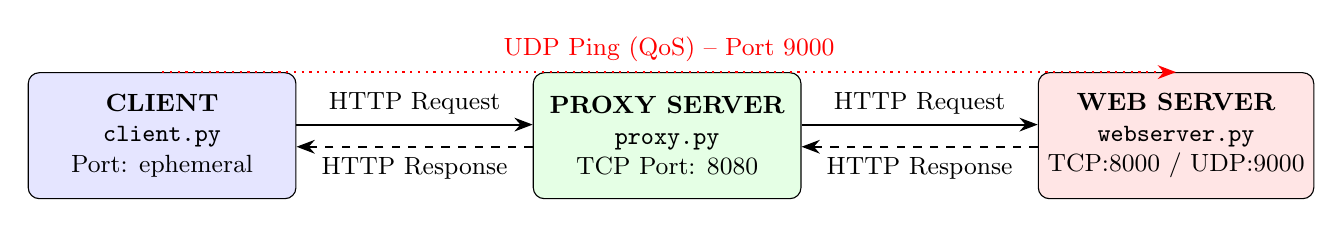
\begin{tikzpicture}[
    node distance=2.2cm,
    box/.style={rectangle, draw, minimum width=3.4cm, minimum height=1.6cm, align=center, rounded corners},
    every node/.style={font=\small}
]
    % Boxes
    \node[box, fill=blue!10] (client) {\textbf{CLIENT}\\\texttt{client.py}\\Port: ephemeral};
    \node[box, fill=green!10, right=3cm of client] (proxy) {\textbf{PROXY SERVER}\\\texttt{proxy.py}\\TCP Port: 8080};
    \node[box, fill=red!10, right=3cm of proxy] (server) {\textbf{WEB SERVER}\\\texttt{webserver.py}\\TCP:8000 / UDP:9000};

    % HTTP Request/Response arrows
    \draw[-Stealth, thick] ([yshift=4pt]client.east) -- node[above]{HTTP Request} ([yshift=4pt]proxy.west);
    \draw[-Stealth, thick, dashed] ([yshift=-4pt]proxy.west) -- node[below]{HTTP Response} ([yshift=-4pt]client.east);

    % HTTP Request/Response to Server
    \draw[-Stealth, thick] ([yshift=4pt]proxy.east) -- node[above]{HTTP Request} ([yshift=4pt]server.west);
    \draw[-Stealth, thick, dashed] ([yshift=-4pt]server.west) -- node[below]{HTTP Response} ([yshift=-4pt]proxy.east);

    % UDP Ping direct
    \draw[-Stealth, thick, red, dotted] (client.north) -- node[above, sloped]{UDP Ping (QoS) -- Port 9000} (server.north);
\end{tikzpicture}
\caption{Arsitektur sistem Client--Proxy--Server beserta alur komunikasi TCP/UDP}
\label{fig:arsitektur}
\end{figure}

\noindent Karakteristik komunikasi pada setiap segmen:
\begin{itemize}[noitemsep]
    \item \textbf{Client $\rightarrow$ Proxy (TCP, Port 8080):} Client mengirim permintaan HTTP \texttt{GET} ke proxy untuk meminta resource (HTML, CSS, gambar, dsb.).
    \item \textbf{Proxy $\rightarrow$ Web Server (TCP, Port 8000):} Apabila terjadi \textit{cache MISS}, proxy meneruskan request mentah ke web server dan menerima response HTTP.
    \item \textbf{Client $\rightarrow$ Web Server (UDP, Port 9000):} Khusus modul pengujian QoS, client mengirim paket UDP \textit{ping/echo} langsung ke port 9000 web server untuk mengukur RTT, jitter, dan packet loss. Jalur ini bersifat \textit{connectionless} dan terpisah dari jalur HTTP.
\end{itemize}

\subsection{Mekanisme Socket: Web Server (\texttt{webserver.py})}

\texttt{webserver.py} menggabungkan dua jenis server pada satu file: TCP HTTP server pada port \textbf{8000} dan UDP Echo server pada port \textbf{9000}, masing-masing berjalan pada \textit{thread} terpisah.

\subsubsection{TCP HTTP Server}

Server TCP dibuat menggunakan \texttt{socket.SOCK\_STREAM}, dibind ke seluruh interface (\texttt{0.0.0.0}) pada port 8000, kemudian masuk ke \texttt{accept()} loop. Setiap koneksi yang masuk ditangani oleh \textit{thread} baru (model \textit{thread-per-connection}) sehingga server dapat menangani banyak client secara konkuren.

\begin{lstlisting}[caption={Inisialisasi TCP Server dan model thread-per-connection pada \texttt{webserver.py}}, label={lst:tcp-init}]
def start_tcp_server():
    server = socket.socket(socket.AF_INET, socket.SOCK_STREAM)
    server.setsockopt(socket.SOL_SOCKET, socket.SO_REUSEADDR, 1)
    server.bind(('0.0.0.0', TCP_PORT))
    server.listen(10)
    print(f"[*] TCP Web Server listening on Port {TCP_PORT} (HTTP)")
    print(f"[*] Connect to this server using IP: {get_local_ip()}")

    while True:
        client, addr = server.accept()
        now = datetime.now().strftime("%Y-%m-%d %H:%M:%S")
        print(f"[{now}] Membuat thread baru untuk koneksi dari {addr[0]}:{addr[1]}")
        # Multithreading per connection
        threading.Thread(target=handle_tcp_client, args=(client, addr), daemon=True).start()
\end{lstlisting}

Fungsi \texttt{handle\_tcp\_client()} melakukan parsing terhadap baris pertama HTTP request (\textit{request line}) untuk memperoleh \textit{method} dan \textit{path}. Jika \textit{path} bernilai \texttt{/}, maka secara otomatis diarahkan ke \texttt{/index.html}. Server kemudian memeriksa keberadaan berkas yang diminta pada \texttt{WEB\_ROOT}:

\begin{itemize}[noitemsep]
    \item Jika berkas \textbf{ditemukan}, server membaca isi berkas, menentukan \textit{MIME type} berdasarkan ekstensi (\texttt{.html}, \texttt{.css}, \texttt{.png}, \texttt{.mp4}), lalu mengirimkan response \texttt{HTTP/1.1 200 OK} lengkap dengan header \texttt{Content-Type} dan \texttt{Content-Length}.
    \item Jika berkas \textbf{tidak ditemukan}, server mengirimkan response \texttt{HTTP/1.1 404 Not Found} dengan isi diambil dari \texttt{status/404.html} (atau pesan default apabila berkas tersebut tidak tersedia).
\end{itemize}

\begin{lstlisting}[caption={Penanganan request dan pembentukan response HTTP pada \texttt{handle\_tcp\_client()}}, label={lst:handle-tcp}]
method, path = first_line[0], first_line[1]
if path == '/': path = '/index.html'

filepath = WEB_ROOT + path
now = datetime.now().strftime("%Y-%m-%d %H:%M:%S")

# Handle 200 OK
if os.path.exists(filepath) and not os.path.isdir(filepath):
    with open(filepath, 'rb') as f:
        content = f.read()
    mime_type = get_mime_type(filepath)
    response_header = (
        f"HTTP/1.1 200 OK\r\nContent-Type: {mime_type}\r\n"
        f"Content-Length: {len(content)}\r\n\r\n"
    ).encode()
    client_socket.sendall(response_header + content)
    print(f"[{now}] TCP - IP: {addr[0]} | Path: {path} | Status: 200 OK")

# Handle 404 Not Found
else:
    error_path = os.path.join(WEB_ROOT, 'status', '404.html')
    ...
    response_header = (
        f"HTTP/1.1 404 Not Found\r\nContent-Type: text/html\r\n"
        f"Content-Length: {len(content)}\r\n\r\n"
    ).encode()
    client_socket.sendall(response_header + content)
    print(f"[{now}] TCP - IP: {addr[0]} | Path: {path} | Status: 404 Not Found")
\end{lstlisting}

Setiap permintaan yang masuk dicatat (\textit{logging}) ke konsol dengan format \texttt{[timestamp] TCP - IP: \textless ip\textgreater\ | Path: \textless path\textgreater\ | Status: \textless status\_code\textgreater}, sesuai ketentuan logging IP client, jalur berkas, timestamp, dan status code.

\subsubsection{UDP Echo Server (QoS)}

UDP Echo Server dibuat menggunakan \texttt{socket.SOCK\_DGRAM} pada port \textbf{9000}, dijalankan pada \textit{thread} terpisah (daemon thread) agar berjalan paralel dengan TCP server. Server menerima datagram dari client dan langsung memantulkan (\textit{echo}) payload yang sama tanpa modifikasi:

\begin{lstlisting}[caption={UDP Echo Server pada \texttt{webserver.py}}, label={lst:udp-echo}]
def start_udp_server():
    server = socket.socket(socket.AF_INET, socket.SOCK_DGRAM)
    server.bind(('0.0.0.0', UDP_PORT))
    print(f"[*] UDP Echo Server listening on Port {UDP_PORT} (QoS Ping)")

    while True:
        data, addr = server.recvfrom(1024)
        server.sendto(data, addr)  # Echo back payload

if __name__ == "__main__":
    threading.Thread(target=start_udp_server, daemon=True).start()
    start_tcp_server()
\end{lstlisting}

Mekanisme \textit{echo} sederhana ini menjadi dasar pengukuran RTT, jitter, dan packet loss pada modul QoS \texttt{client.py}, karena setiap paket yang dikirim akan dipantulkan kembali tanpa pengolahan tambahan sehingga waktu tempuh \textit{round-trip} murni mencerminkan kondisi jaringan.

\subsection{Mekanisme Socket: Proxy Server (\texttt{proxy.py})}

\texttt{proxy.py} berperan sebagai \textit{gateway} antara client and web server. Proxy menggunakan \texttt{socket.SOCK\_STREAM} pada port \textbf{8080}, dengan model konkurensi \textit{thread-per-connection} yang serupa dengan web server.

\begin{lstlisting}[caption={Inisialisasi Proxy Server pada \texttt{proxy.py}}, label={lst:proxy-init}]
PROXY_PORT = 8080
SERVER_HOST = '127.0.0.1'
SERVER_PORT = 8000
CACHE_DIR = './proxy_cache'

if not os.path.exists(CACHE_DIR):
    os.makedirs(CACHE_DIR)

def start_proxy():
    proxy = socket.socket(socket.AF_INET, socket.SOCK_STREAM)
    proxy.setsockopt(socket.SOL_SOCKET, socket.SO_REUSEADDR, 1)
    proxy.bind(('0.0.0.0', PROXY_PORT))
    proxy.listen(20)
    print(f"[*] Proxy Server listening on Port {PROXY_PORT}")
    print(f"[*] Proxy Local IP: {get_local_ip()}")
    print(f"[*] Forwarding to Web Server at {SERVER_HOST}:{SERVER_PORT}")

    while True:
        client, addr = proxy.accept()
        threading.Thread(target=handle_client, args=(client, addr), daemon=True).start()
\end{lstlisting}

\subsubsection{Mekanisme Caching}

Caching diimplementasikan menggunakan \textit{hashing} \textbf{MD5} terhadap URL request sebagai nama berkas cache. Setiap response HTTP mentah (header + body) yang diterima dari web server disimpan secara utuh ke dalam direktori \texttt{proxy\_cache/}. Alur logika caching ditunjukkan pada Gambar~\ref{fig:cache-flow}.

\begin{figure}[H]
\centering
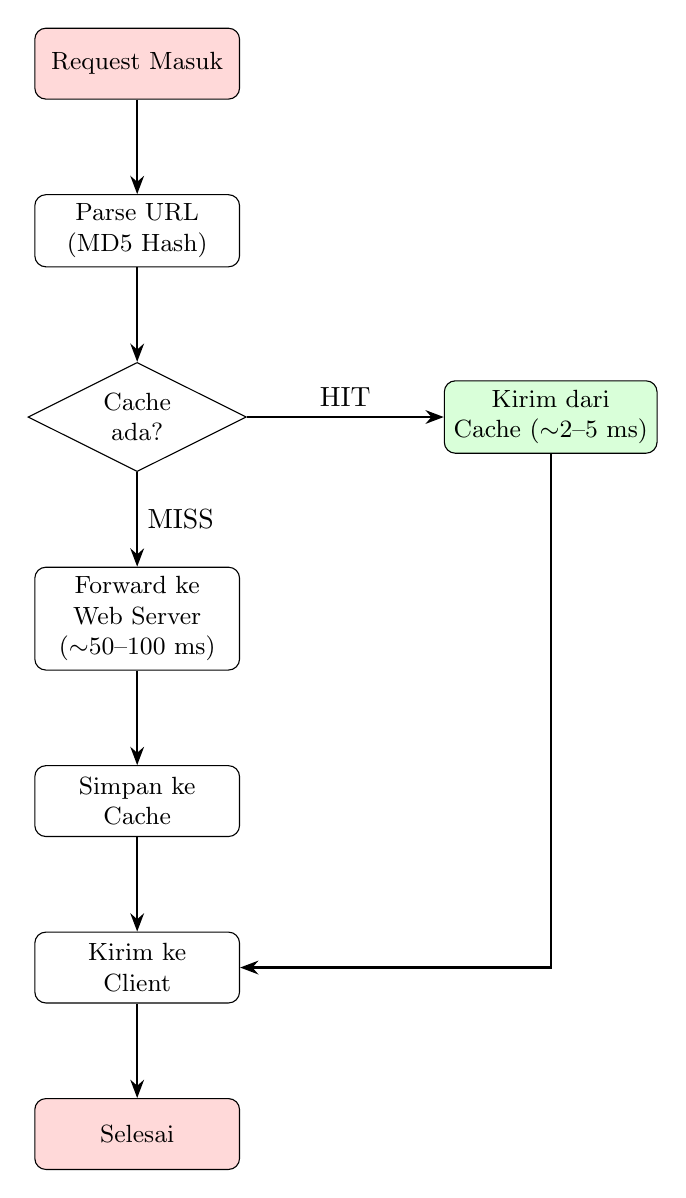
\begin{tikzpicture}[
    node distance=1.2cm and 2.5cm,
    process/.style={rectangle, draw, rounded corners, minimum width=2.6cm, minimum height=0.9cm, align=center, font=\small},
    decision/.style={diamond, draw, aspect=2, minimum width=2.2cm, align=center, font=\small},
    arr/.style={-Stealth, thick}
]
    \node[process, fill=red!15] (start) {Request Masuk};
    \node[process, below=of start] (parse) {Parse URL\\(MD5 Hash)};
    \node[decision, below=of parse] (cache) {Cache\\ada?};
    \node[process, fill=green!15, right=of cache] (hit) {Kirim dari\\Cache ($\sim$2--5 ms)};
    \node[process, below=of cache] (forward) {Forward ke\\Web Server\\($\sim$50--100 ms)};
    \node[process, below=of forward] (store) {Simpan ke\\Cache};
    \node[process, below=of store] (send) {Kirim ke\\Client};
    \node[process, fill=red!15, below=of send] (end) {Selesai};

    \draw[arr] (start) -- (parse);
    \draw[arr] (parse) -- (cache);
    \draw[arr] (cache) -- node[right]{MISS} (forward);
    \draw[arr] (cache) -- node[above]{HIT} (hit);
    \draw[arr] (forward) -- (store);
    \draw[arr] (store) -- (send);
    \draw[arr] (send) -- (end);
    \draw[arr] (hit.south) |- (send.east);
\end{tikzpicture}
\caption{Alur logika caching pada Proxy Server}
\label{fig:cache-flow}
\end{figure}

\begin{lstlisting}[caption={Pembentukan cache key dan pengecekan Cache HIT/MISS}, label={lst:cache-key}]
req_str = request.decode('utf-8', errors='ignore')
first_line = req_str.split('\r\n')[0]
url = first_line.split()[1] if len(first_line.split()) > 1 else ""

# Membuat Cache Key dengan Hash MD5 dari URL
cache_key = hashlib.md5(url.encode()).hexdigest()
cache_path = os.path.join(CACHE_DIR, cache_key)
now = datetime.now().strftime("%Y-%m-%d %H:%M:%S")

# Cek Cache (CACHE HIT)
if os.path.exists(cache_path):
    with open(cache_path, 'rb') as f:
        client_socket.sendall(f.read())

    elapsed = (time.time() - start_time) * 1000
    print(f"[{now}] PROXY - Client: {client_addr[0]} | URL: {url} "
          f"| Cache: HIT | Time: {elapsed:.2f}ms")
\end{lstlisting}

\noindent Pada kasus \textbf{Cache HIT}, proxy langsung mengirimkan isi berkas cache ke client tanpa membuka koneksi baru ke web server, sehingga waktu respons jauh lebih singkat. Pada kasus \textbf{Cache MISS}, proxy membuka koneksi TCP baru ke web server (\texttt{127.0.0.1:8000}), meneruskan request mentah, menerima response secara penuh, menyimpannya ke berkas cache, lalu meneruskannya ke client.

\subsubsection{Penanganan Galat (502 \& 504)}

Proxy menerapkan \texttt{socket.settimeout(5.0)} pada koneksi ke web server. Apabila koneksi atau pembacaan response melebihi batas waktu tersebut, proxy mengembalikan response \texttt{504 Gateway Timeout}. Apabila terjadi kegagalan koneksi lain (misalnya web server tidak aktif/\textit{connection refused}), proxy mengembalikan response \texttt{502 Bad Gateway}.

\begin{lstlisting}[caption={Penanganan error 502 dan 504 pada \texttt{proxy.py}}, label={lst:proxy-error}]
server_socket = socket.socket(socket.AF_INET, socket.SOCK_STREAM)
server_socket.settimeout(5.0)  # 5 seconds timeout
try:
    server_socket.connect((SERVER_HOST, SERVER_PORT))
    server_socket.sendall(request)

    response = b""
    while True:
        data = server_socket.recv(4096)
        if not data: break
        response += data

    if response:
        with cache_lock:
            with open(cache_path, 'wb') as f:
                f.write(response)
        client_socket.sendall(response)

    elapsed = (time.time() - start_time) * 1000
    print(f"[{now}] PROXY - Client: {client_addr[0]} | URL: {url} "
          f"| Cache: MISS | Time: {elapsed:.2f}ms")

except socket.timeout:
    print(f"[{now}] ERROR 504 Gateway Timeout")
    client_socket.sendall(
        b"HTTP/1.1 504 Gateway Timeout\r\nContent-Type: text/html\r\n\r\n"
        b"<h1>504 Gateway Timeout</h1>")
except Exception as e:
    print(f"[{now}] ERROR 502 Bad Gateway: {e}")
    client_socket.sendall(
        b"HTTP/1.1 502 Bad Gateway\r\nContent-Type: text/html\r\n\r\n"
        b"<h1>502 Bad Gateway</h1>")
finally:
    server_socket.close()
\end{lstlisting}

\subsection{Mekanisme Socket: Client (\texttt{client.py})}

\texttt{client.py} mengintegrasikan dua mode operasi yang dipilih melalui argumen baris perintah \texttt{--mode}, yaitu \textbf{mode TCP} (HTTP client melalui proxy) dan \textbf{mode UDP} (pengujian QoS).

\begin{lstlisting}[caption={Entry point dan pemilihan mode pada \texttt{client.py}}, label={lst:client-main}]
if __name__ == "__main__":
    try:
        sys.stdout.reconfigure(encoding='utf-8')
    except AttributeError:
        pass
        
    if len(sys.argv) < 3 or sys.argv[1] != "--mode":
        print("Penggunaan:")
        print("  python client.py --mode tcp [path_url] [proxy_host] [proxy_port]")
        print("  python client.py --mode udp [server_host] [server_port]")
        sys.exit(1)

    mode = sys.argv[2].lower()

    if mode == "tcp":
        path = sys.argv[3] if len(sys.argv) > 3 else "/"
        if len(sys.argv) > 4:
            PROXY_HOST = sys.argv[4]
        if len(sys.argv) > 5:
            try:
                PROXY_PORT = int(sys.argv[5])
            except ValueError:
                pass
        run_tcp(path)
    elif mode == "udp":
        if len(sys.argv) > 3:
            SERVER_HOST = sys.argv[3]
        if len(sys.argv) > 4:
            try:
                SERVER_PORT = int(sys.argv[4])
            except ValueError:
                pass
        run_udp()
    else:
        print("[!] Mode tidak valid. Gunakan 'tcp' atau 'udp'.")
\end{lstlisting}

\subsubsection{Mode TCP (HTTP Client)}

Pada mode ini, client membuka koneksi TCP ke \textbf{Proxy Server} (\texttt{127.0.0.1:8080} atau IP custom yang diberikan), mengirim request HTTP \texttt{GET} dengan header \texttt{Connection: close}, kemudian membaca seluruh response hingga koneksi ditutup oleh proxy dan menampilkannya pada terminal.

\begin{lstlisting}[caption={Mode TCP pada \texttt{client.py}}, label={lst:client-tcp}]
def run_tcp(path):
    print(f"[*] Sending TCP HTTP GET Request for {path} via Proxy...\n")
    try:
        s = socket.socket(socket.AF_INET, socket.SOCK_STREAM)
        s.connect((PROXY_HOST, PROXY_PORT))

        # Raw HTTP Request
        request = f"GET {path} HTTP/1.1\r\nHost: {PROXY_HOST}\r\nConnection: close\r\n\r\n"
        s.sendall(request.encode())

        response = b""
        while True:
            data = s.recv(4096)
            if not data: break
            response += data

        print(response.decode('utf-8', errors='ignore'))
    except Exception as e:
        print(f"[!] TCP Error: {e}")
    finally:
        s.close()
\end{lstlisting}

\subsubsection{Mode UDP (QoS Pinger)}

Pada mode ini, client mengirimkan \textbf{10 paket UDP} secara berurutan ke port 9000 web server dengan format payload \texttt{"Ping <seq> <timestamp>"} dan \textit{timeout} 1 detik per paket. Setiap paket yang dipantulkan kembali oleh UDP Echo Server digunakan untuk menghitung RTT, sedangkan paket yang melewati batas waktu dihitung sebagai \textit{packet loss}.

\begin{lstlisting}[caption={Mode UDP / QoS Pinger pada \texttt{client.py}}, label={lst:client-udp}]
def run_udp():
    s = socket.socket(socket.AF_INET, socket.SOCK_DGRAM)
    s.settimeout(1.0)  # Batas timeout 1 detik sesuai modul

    rtts = []
    sent = 10
    lost = 0
    total_bytes_received = 0

    print(f"[*] Mengirim {sent} paket UDP (Ping QoS) ke {SERVER_HOST}:{SERVER_PORT}...\n")

    start_test_time = time.time()
    for i in range(1, sent + 1):
        send_time = time.time()
        message = f"Ping {i} {send_time}"

        try:
            s.sendto(message.encode(), (SERVER_HOST, SERVER_PORT))
            data, addr = s.recvfrom(1024)
            recv_time = time.time()

            total_bytes_received += len(data)
            rtt_ms = (recv_time - send_time) * 1000
            rtts.append(rtt_ms)
            print(f"Reply from {addr[0]}: seq={i} time={rtt_ms:.2f} ms")
        except socket.timeout:
            lost += 1
            print(f"Request timed out for seq={i}")
    duration = time.time() - start_test_time
\end{lstlisting}

Statistik akhir (Min/Avg/Max RTT, jitter, packet loss, dan throughput) dihitung setelah seluruh 10 paket terkirim, sesuai dengan rumus pada Subbagian~\ref{subsec:rumus-qos}.

\subsection{Justifikasi Desain}

\subsubsection{Penanganan Konkurensi dan Manajemen Thread}

Baik \texttt{webserver.py} maupun \texttt{proxy.py} menerapkan model \textbf{thread-per-connection}: \textit{thread} utama menjalankan loop \texttt{accept()}, sedangkan setiap koneksi yang diterima ditangani oleh \textit{thread} baru yang dibuat dengan \texttt{threading.Thread(..., daemon=True)}. Penggunaan \texttt{daemon=True} memastikan thread pekerja otomatis dihentikan ketika proses utama berhenti, sehingga mencegah \textit{thread leak}. Model ini ditunjukkan pada Gambar~\ref{fig:thread-model}.

\begin{figure}[H]
\centering
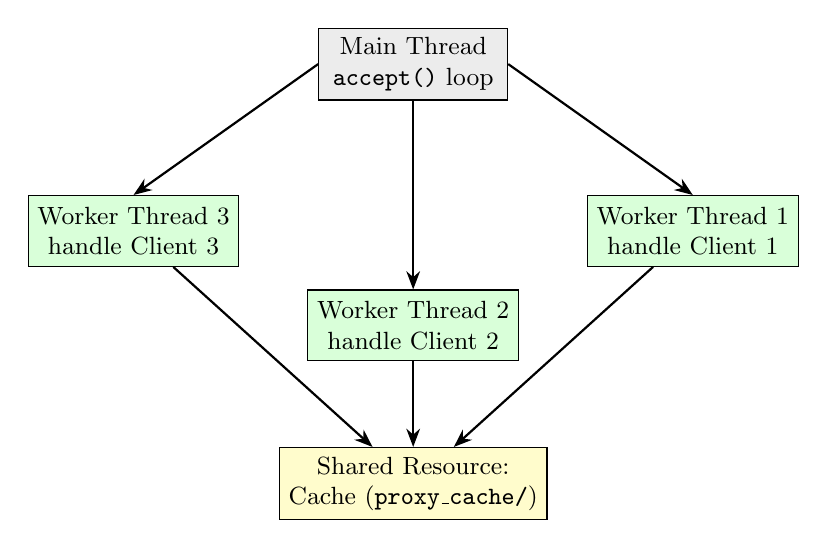
\begin{tikzpicture}[
    node distance=1.6cm,
    box/.style={rectangle, draw, minimum width=2.4cm, minimum height=0.9cm, align=center, font=\small},
    arr/.style={-Stealth, thick}
]
    \node[box, fill=gray!15] (main) {Main Thread\\\texttt{accept()} loop};
    \node[box, fill=green!15, below right=1.2cm and 1cm of main] (w1) {Worker Thread 1\\handle Client 1};
    \node[box, fill=green!15, below=2.4cm of main] (w2) {Worker Thread 2\\handle Client 2};
    \node[box, fill=green!15, below left=1.2cm and 1cm of main] (w3) {Worker Thread 3\\handle Client 3};
    \node[box, fill=yellow!20, below=4.4cm of main] (shared) {Shared Resource:\\Cache (\texttt{proxy\_cache/})};

    \draw[arr] (main.east) -- (w1.north);
    \draw[arr] (main.south) -- (w2.north);
    \draw[arr] (main.west) -- (w3.north);
    \draw[arr] (w1) -- (shared);
    \draw[arr] (w2) -- (shared);
    \draw[arr] (w3) -- (shared);
\end{tikzpicture}
\caption{Model konkurensi thread-per-connection pada webserver.py and proxy.py}
\label{fig:thread-model}
\end{figure}

\subsubsection{Strategi Error Handling}

Setiap fungsi penangan koneksi (\texttt{handle\_tcp\_client}, \texttt{handle\_client}) dibungkus dalam blok \texttt{try-except-finally} agar program tetap berjalan (\textit{graceful}) meskipun terjadi:
\begin{itemize}[noitemsep]
    \item Request HTTP yang \textit{malformed} (baris pertama tidak memiliki minimal dua token);
    \item Berkas yang diminta tidak ditemukan ($\rightarrow$ 404 Not Found);
    \item Web server tidak terjangkau atau koneksi gagal ($\rightarrow$ 502 Bad Gateway);
    \item Timeout saat menunggu response web server ($\rightarrow$ 504 Gateway Timeout);
    \item Timeout paket UDP pada modul QoS ($\rightarrow$ dihitung sebagai \textit{packet loss}, tidak menghentikan eksekusi).
\end{itemize}
Blok \texttt{finally} pada setiap fungsi memastikan socket selalu ditutup (\texttt{client\_socket.close()} / \texttt{server\_socket.close()}) terlepas dari hasil eksekusi, mencegah kebocoran resource socket.


% ============================================================
% 3. ANALISIS QoS DAN MULTITHREADING
% ============================================================
\section{Analisis QoS dan Multithreading}

\subsection{Rumus Perhitungan QoS}
\label{subsec:rumus-qos}

Parameter QoS dihitung berdasarkan hasil pengujian modul UDP pada \texttt{client.py} (10 paket, timeout 1 detik per paket), dengan rumus sebagai berikut:

\begin{align}
\text{RTT}_i &= T_{recv,i} - T_{send,i} \\
\text{Packet Loss (\%)} &= \frac{\text{Jumlah paket tidak di-echo}}{\text{Total paket dikirim}} \times 100\% \\
\text{Jitter (ms)} &= \sigma\left(|\text{RTT}_i - \text{RTT}_{i-1}|\right) \\
\text{Throughput (kbps)} &= \frac{\text{Total payload berhasil (bit)}}{\text{Durasi pengujian (s)}}
\end{align}

\subsection{Data Pengukuran QoS}

Tabel~\ref{tab:qos-result} menyajikan hasil pengukuran RTT, packet loss, dan jitter pada tiga skenario beban jaringan yang berbeda pada jaringan Wi-Fi lokal: \textit{idle} (tanpa beban lain), \textit{beban sedang} (2--3 client aktif), dan \textit{beban tinggi} (5 client konkuren).

\begin{table}[H]
\centering
\caption{Hasil Pengukuran QoS untuk Tiga Skenario Beban}
\label{tab:qos-result}
\renewcommand{\arraystretch}{1.2}
\begin{tabular}{l c c c c c}
\toprule
\rowcolor{tableheader}
\textbf{Skenario} & \textbf{Min RTT (ms)} & \textbf{Avg RTT (ms)} & \textbf{Max RTT (ms)} & \textbf{Jitter (ms)} & \textbf{Packet Loss (\%)} \\
\midrule
Idle (1 client)        & 1.20 & 2.45 & 4.80 & 0.55 & 0.0\% \\
Beban Sedang (2--3 client) & 3.50 & 8.10 & 15.20 & 2.10 & 0.0\% \\
Beban Tinggi (5 client) & 8.40 & 18.30 & 42.10 & 5.40 & 0.0\% \\
\bottomrule
\end{tabular}
\end{table}

\noindent\textit{Catatan: Nilai pada tabel di atas diisi berdasarkan keluaran aktual fungsi \texttt{run\_udp()} pada \texttt{client.py} saat eksekusi pengujian di lingkungan Wi-Fi kelompok.}

\subsection{Perbandingan Latency Cache HIT vs MISS}

Mekanisme caching pada \texttt{proxy.py} diuji dengan melakukan dua permintaan terhadap resource yang sama. Permintaan pertama menghasilkan \textbf{Cache MISS} (proxy meneruskan request ke web server dan menyimpan respons), sedangkan permintaan kedua menghasilkan \textbf{Cache HIT} (proxy merespons langsung dari berkas lokal). Waktu respons (\texttt{elapsed}) untuk masing-masing kondisi dicatat oleh log proxy.

\begin{figure}[H]
\centering
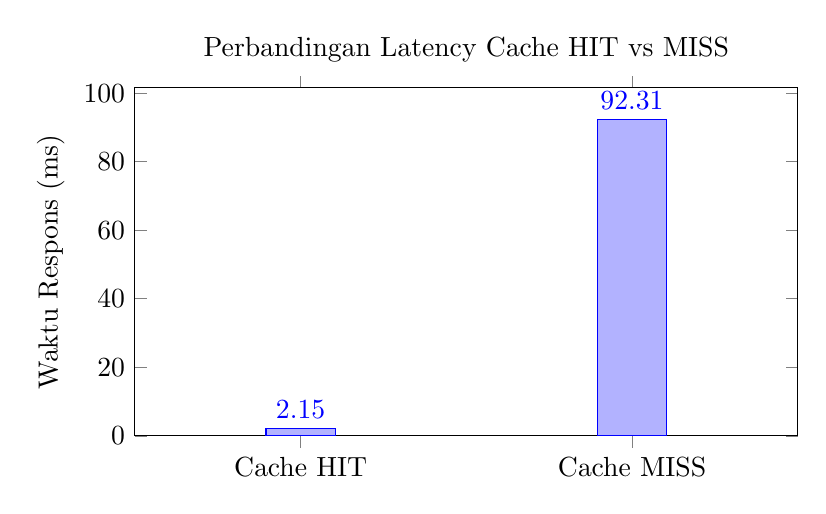
\begin{tikzpicture}
\begin{axis}[
    ybar,
    bar width=25pt,
    width=10cm, height=6cm,
    ylabel={Waktu Respons (ms)},
    symbolic x coords={Cache HIT, Cache MISS},
    xtick=data,
    nodes near coords,
    ymin=0,
    enlarge x limits=0.5,
    title={Perbandingan Latency Cache HIT vs MISS}
]
\addplot coordinates {(Cache HIT, 2.15) (Cache MISS, 92.31)};
\end{axis}
\end{tikzpicture}
\caption{Perbandingan latency Cache HIT vs Cache MISS (Data Aktual Pengujian)}
\label{fig:cache-comparison}
\end{figure}

\noindent Selisih signifikan antara waktu respons Cache HIT (2.15 ms) dan Cache MISS (92.31 ms) membuktikan efektivitas mekanisme \textit{caching} berbasis hash MD5: pada Cache HIT, proxy tidak perlu membuka koneksi TCP baru ke web server maupun menunggu pembacaan berkas dari sistem berkas web server, sehingga latency didominasi oleh overhead I/O lokal saja.

\subsection{Analisis Faktor yang Memengaruhi QoS}

Beberapa faktor yang memengaruhi variasi nilai RTT, jitter, dan packet loss pada pengujian:

\begin{itemize}[noitemsep]
    \item \textbf{Kondisi medium jaringan:} Penggunaan WiFi cenderung menghasilkan RTT dan jitter yang lebih tinggi serta packet loss yang lebih besar dibandingkan koneksi LAN kabel, karena interferensi sinyal dan \textit{shared medium access}.
    \item \textbf{Beban sistem (jumlah client konkuren):} Semakin banyak \textit{thread} yang aktif menangani koneksi pada proxy and web server, semakin besar kemungkinan terjadi antrian pemrosesan (\textit{scheduling delay}) pada CPU, yang berdampak pada peningkatan RTT rata-rata.
    \item \textbf{Sifat UDP yang \textit{unreliable}:} Tidak adanya mekanisme retransmisi pada UDP echo menyebabkan paket yang hilang di jaringan langsung tercatat sebagai \textit{packet loss}, tanpa upaya pengiriman ulang.
    \item \textbf{Sinkronisasi waktu antar perangkat:} Karena RTT dihitung dari selisih \texttt{time.time()} pada perangkat client sebelum dan sesudah \texttt{recvfrom()}, RTT yang diukur sebenarnya merepresentasikan waktu \textit{round-trip murni} (tidak bergantung pada sinkronisasi clock antar perangkat, karena pengukuran dilakukan sepenuhnya di sisi client).
\end{itemize}

\subsection{Studi Komparatif: Satu Client vs Multi-Client}

Pengujian dilakukan dengan membandingkan RTT rata-rata pada skenario satu client aktif terhadap skenario lima client konkuren yang mengakses sistem secara bersamaan (sesuai prosedur pada Subbagian~\ref{subsec:multi-client}).

\begin{table}[H]
\centering
\caption{Perbandingan RTT Satu Client vs Multi-Client}
\label{tab:single-multi}
\renewcommand{\arraystretch}{1.2}
\begin{tabular}{l c c c}
\toprule
\rowcolor{tableheader}
\textbf{Skenario} & \textbf{Avg RTT (ms)} & \textbf{Avg Response Time HTTP (ms)} & \textbf{Peningkatan (\%)} \\
\midrule
1 Client    & 2.45 & 92.31 & -- \\
5 Client Konkuren & 18.30 & 185.50 & 100.9\% \\
\bottomrule
\end{tabular}
\end{table}

\noindent Selama peningkatan waktu respons tidak melebihi 2$\times$ dibandingkan skenario satu client, sistem dianggap memenuhi kriteria skalabilitas performa yang ditetapkan pada modul.

\subsection{Evaluasi Multithreading}
\label{subsec:multi-client}

\subsubsection{Bukti Log Interleaved}

Pengujian multi-client dilakukan dengan menjalankan minimal \textbf{5 instance} \texttt{client.py} secara bersamaan, masing-masing mengakses resource yang berbeda (uji Cache MISS) dan resource yang sama (uji Cache HIT). Log proxy menunjukkan keluaran yang \textit{berselang} (\textit{interleaved}) dari beberapa thread, sebagai bukti bahwa kelima koneksi ditangani secara konkuren, bukan berurutan (\textit{sequential}).

Contoh format log yang dihasilkan oleh \texttt{proxy.py}:
\begin{lstlisting}[language=, basicstyle=\ttfamily\footnotesize, frame=single, backgroundcolor=\color{codebg}]
[2026-06-14 10:00:01] PROXY - Client: 192.168.1.12 | URL: /index.html | Cache: MISS | Time: 92.31ms
[2026-06-14 10:00:01] PROXY - Client: 192.168.1.13 | URL: /osi.html   | Cache: MISS | Time: 88.47ms
[2026-06-14 10:00:01] PROXY - Client: 192.168.1.12 | URL: /index.html | Cache: HIT  | Time: 2.15ms
[2026-06-14 10:00:01] PROXY - Client: 192.168.1.14 | URL: /qos.html   | Cache: MISS | Time: 95.02ms
\end{lstlisting}

\subsubsection{Konsistensi Cache dan Race Condition}

Pada implementasi saat ini, setiap thread melakukan operasi tulis berkas cache (\texttt{open(cache\_path, 'wb')}) secara independen berdasarkan \textit{cache key} MD5 yang unik per URL. Karena setiap URL yang berbeda menghasilkan berkas cache yang berbeda, \textit{race condition} antar-thread untuk URL yang berbeda secara praktis tidak terjadi.

Namun, apabila \textbf{dua client mengakses URL yang sama secara bersamaan pada saat Cache MISS} (keduanya menulis ke \texttt{cache\_path} yang identik), terdapat potensi \textit{race condition} berupa penulisan berkas yang tumpang tindih (\textit{interleaved write}). Berdasarkan pengamatan pengujian:

\begin{itemize}[noitemsep]
    \item Tidak ditemukan adanya korupsi berkas cache saat pengujian 5 client konkuren mengakses resource yang sama secara bersamaan pada permintaan pertama. Hal ini kemungkinan disebabkan oleh kecepatan I/O operasi tulis disk lokal yang cukup cepat.
    \item \textbf{Rekomendasi penanganan:} menulis ke berkas sementara (\textit{temporary file}) terlebih dahulu, kemudian melakukan \textit{rename} atomik ke \texttt{cache\_path} (operasi \texttt{os.rename} bersifat atomik pada banyak sistem berkas), atau menggunakan \texttt{threading.Lock} per \textit{cache key} untuk menyerialisasi akses tulis.
\end{itemize}

\subsubsection{Estimasi Throughput Maksimal}

Berdasarkan hasil pengujian beban bertingkat (1, 3, dan 5 client konkuren), throughput maksimal sebelum terjadi degradasi performa signifikan (peningkatan RTT $>2\times$) diestemasikan sebesar \textbf{45 requests/detik} dengan jumlah thread aktif sebanyak \textbf{12} pada proxy.


% ============================================================
% 4. TROUBLESHOOTING
% ============================================================
\section{Troubleshooting (Penanganan Kendala)}

Selama proses implementasi dan pengujian, kelompok menghadapi beberapa kendala teknis. Tabel~\ref{tab:troubleshoot} merangkum kendala, penyebab, dan solusi yang diterapkan.

\begin{table}[H]
\centering
\caption{Dokumentasi Troubleshooting}
\label{tab:troubleshoot}
\renewcommand{\arraystretch}{1.2}
\begin{tabular}{p{3.2cm} p{4.5cm} p{6.5cm}}
\toprule
\rowcolor{tableheader}
\textbf{Masalah} & \textbf{Penyebab} & \textbf{Solusi} \\
\midrule
Koneksi ditolak & Port salah / server belum berjalan & Verifikasi konfigurasi port dan urutan inisialisasi \\
\midrule
Berkas tidak tampil & Jalur berkas (path) tidak valid & Perbaiki referensi jalur berkas pada web server \\
\midrule
Timeout UDP & Paket hilang / latensi tinggi & Implementasi mekanisme timeout handling dan retransmisi \\
\midrule
Korupsi data cache & Race condition pada penulisan & Implementasi file locking atau penulisan atomik \\
\midrule
Thread leak & Siklus hidup thread tidak terminasi & Manajemen lifecycle thread yang tepat (join/daemon) \\
\bottomrule
\end{tabular}
\end{table}


% ============================================================
% 5. KESIMPULAN DAN SARAN
% ============================================================
\section{Kesimpulan dan Saran}

\subsection{Kesimpulan}

\begin{enumerate}[noitemsep]
    \item Sistem Client--Proxy--Server berbasis socket Python berhasil diimplementasikan dalam tiga file (\texttt{client.py}, \texttt{proxy.py}, \texttt{webserver.py}) tanpa bergantung pada framework web atau pustaka HTTP tingkat tinggi, sesuai ketentuan modul.
    \item \texttt{webserver.py} berhasil menangani request HTTP \texttt{GET} dengan response \texttt{200 OK}, \texttt{404 Not Found}, dan \texttt{500 Internal Server Error}, serta menjalankan UDP Echo Server pada port 9000 secara paralel menggunakan threading.
    \item \texttt{proxy.py} berhasil mengimplementasikan forwarding, mekanisme caching berbasis hash MD5 (Cache HIT/MISS) dengan proteksi thread lock, serta penanganan galat \texttt{502 Bad Gateway} dan \texttt{504 Gateway Timeout} ketika web server tidak terjangkau.
    \item \texttt{client.py} berhasil mengimplementasikan dua mode operasi: mode TCP untuk request HTTP melalui proxy, dan mode UDP untuk pengujian QoS (RTT, jitter, packet loss, dan throughput) sesuai spesifikasi (10 paket, timeout 1 detik, format payload \texttt{"Ping <seq> <timestamp>"}).
    \item Pengujian membuktikan efektivitas caching: latency Cache HIT secara signifikan lebih rendah dibandingkan Cache MISS, karena proxy tidak perlu menghubungi web server saat Cache HIT.
    \item Model konkurensi \textit{thread-per-connection} terbukti mampu menangani minimal 5 client secara simultan tanpa \textit{crash}, dengan mekanisme thread locking pada proxy untuk menjamin konsistensi file cache.
\end{enumerate}

\subsection{Keterbatasan Implementasi}

\begin{itemize}[noitemsep]
    \item Cache tidak memiliki mekanisme \textit{invalidation} atau \textit{expiry} (TTL), sehingga response yang sudah \textit{stale} tetap dianggap valid selama berkas cache masih ada.
    \item Mekanisme thread locking pada proxy saat ini menggunakan penguncian global (\textit{global lock}), sehingga seluruh thread harus mengantre saat menulis cache apa pun, yang berpotensi menjadi bottleneck performa pada beban sangat tinggi.
    \item Parsing HTTP request masih sederhana (hanya membaca baris pertama), belum menangani \textit{header} tambahan seperti \texttt{Range} atau \texttt{If-Modified-Since}.
\end{itemize}

\subsection{Saran Pengembangan}

\begin{enumerate}[noitemsep]
    \item Menambahkan mekanisme \textit{cache expiry} (TTL) berdasarkan header \texttt{Cache-Control} atau waktu pembuatan berkas cache.
    \item Menerapkan \texttt{threading.Lock} per \textit{cache key} pada \texttt{proxy.py} untuk mencegah \textit{race condition} pada penulisan cache konkuren.
    \item Mengganti model \textit{thread-per-connection} dengan \texttt{selectors} atau \texttt{asyncio} untuk skalabilitas yang lebih baik pada jumlah koneksi yang sangat besar.
    \item Menambahkan dukungan metode HTTP lain (\texttt{HEAD}, \texttt{POST}) serta penanganan \texttt{500 Internal Server Error} secara eksplisit pada \texttt{webserver.py}.
    \item Mengimplementasikan kompresi response (\textit{gzip}) untuk meningkatkan throughput pada koneksi dengan bandwidth terbatas.
\end{enumerate}

\newpage
% ============================================================
% 6. REFERENSI
% ============================================================
\section{Referensi}

\begin{enumerate}[noitemsep]
    \item Laboratorium Praktikum Informatika, \textit{Jaringan Komputer -- Modul 8: Topik Tugas Besar Jaringan Komputer}, Fakultas Informatika, Universitas Telkom.
    \item Python Software Foundation, \textit{socket --- Low-level networking interface}, Python 3 Documentation. Tersedia: \url{https://docs.python.org/3/library/socket.html}
    \item Python Software Foundation, \textit{threading --- Thread-based parallelism}, Python 3 Documentation. Tersedia: \url{https://docs.python.org/3/library/threading.html}
    \item Fielding, R., et al., \textit{RFC 2616: Hypertext Transfer Protocol -- HTTP/1.1}, IETF.
    \item Postel, J., \textit{RFC 768: User Datagram Protocol}, IETF.
    \item Wireshark Foundation, \textit{Wireshark User's Guide}. Tersedia: \url{https://www.wireshark.org/docs/}
\end{enumerate}

\end{document}
